\documentclass{article}
\usepackage{fontspec}
\usepackage{polyglossia}
\setdefaultlanguage{french}
\usepackage[a4paper,margin=3cm]{geometry}

\usepackage{amsmath}
\usepackage{amssymb}
\usepackage{array}
\usepackage{auto-pst-pdf}
\usepackage{booktabs}
\usepackage{cite}
\usepackage{graphicx}
\usepackage{lmodern}
\usepackage{marvosym}
\usepackage{mathrsfs}
\usepackage{minted}
\usepackage{multicol}
\usepackage{multirow}
\usepackage{paralist}
\usepackage{schemabloc}
\usepackage{siunitx}
\usepackage{soul}
\usepackage{tikz}
\usepackage[european,cuteinductors,siunitx]{circuitikz}
\usepackage{url,hyperref}
\usepackage{verbatim}
\usepackage{xunicode,xltxtra}

\title{
\includegraphics{../../../images/inp-enseeiht} \\ ~ \\ ~ \\ ~ \\ ~ \\ Rapport CCMB}
\author{François Pierron \& Guilhem Saurel}
\date{\oldstylenums{\today}}

\begin{document}

\begin{titlepage}
    \setcounter{page}{0}
    \maketitle
    \vfill
    \tableofcontents
    \thispagestyle{empty}
\end{titlepage}

\section*{Introduction}

L’objectif de ce TP est de partir d’un circuit idéal connu, et de remplacer petit à petit les composants idéaux les plus sensibles à un milieu bruité par des modélisation des composants réels.

~

On espère donc observer des dégradations des résultats, mais qui restent faibles voire négligeable. Si elles deviennent trop importantes, il nous faudra trouver des solutions afin de limiter les effets néfastes du milieu bruité.


\section{Circuit initial}
Notre circuit initial est un simple amplificateur à émetteur commun:

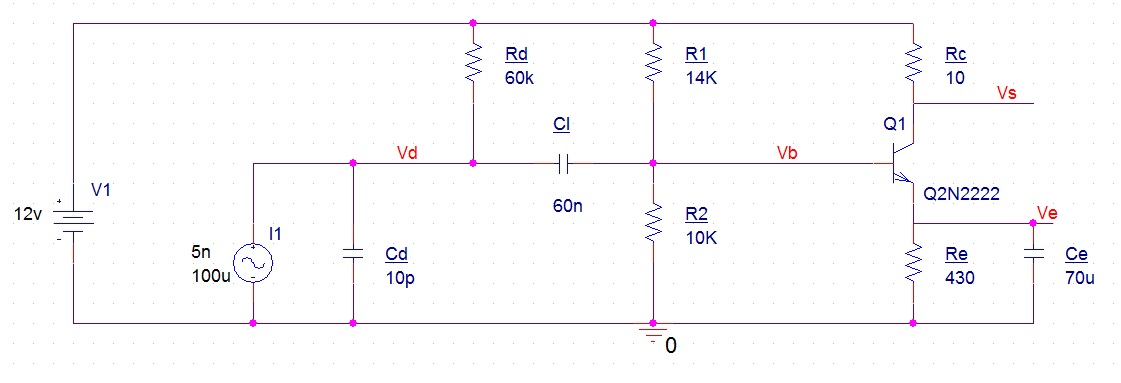
\includegraphics[width=\linewidth]{schema_ideal.jpg}

Son diagramme de Bode est le suivant:

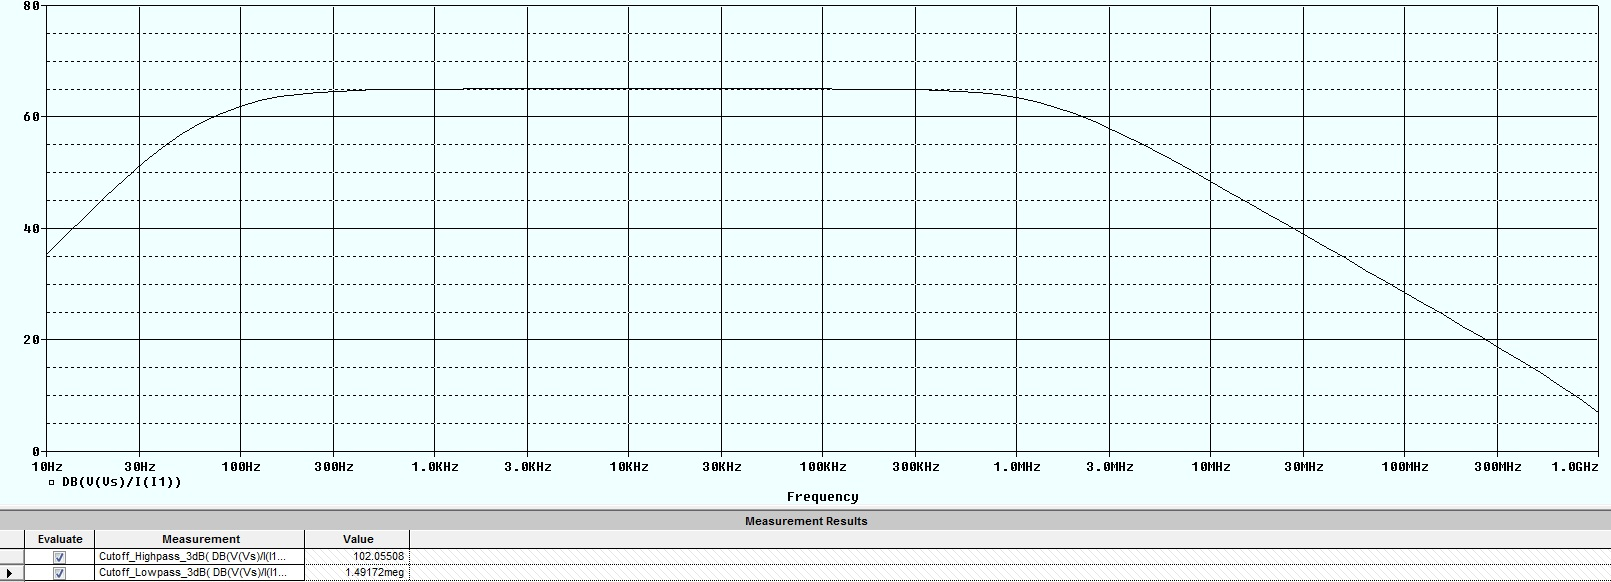
\includegraphics[width=\linewidth]{bode_ideal.jpg}

%Notre fréquence de coupure basse se site aux alentours de 40Hz, ce qui est bien inférieur au 100Hz demandés, et notre fréquence de coupure haute est aux alentours de 70MHz, ce qui est supérieur aux 10MHz attendus.

Notre fréquence de coupure basse est de 102Hz, et la fréquence de coupure haute est de 1.49MHz.

(Pour des raisons matérielles, nous n’avons pas pu prendre le transistor initialement prévu dans le sujet).

\section{Modélisation des condensateurs réels}

Parmis nos composants, on remarque que les condensateurs seront très sensibles au bruit, on va donc les remplacer par un modèle plus proche de la réalité telle que décrite dans les datasheet de condensateurs qu’on choisira sur le internet.

On a d’abord besoin d’un condensateur de 47µF. On va donc chercher la datasheet du moins cher sur Farnell qui accepte notre tension. On tombe sur le EEEFK1C470UR qui a une résistance série de 0.36Ω. Cette datasheet ne renseigne pas de fréquence de résonnance ni d’ESL, donc nous devons nous contenter de cette résistance supplémentaire.

On remarque que nos fréquences de coupure sont très légèrement décalées:

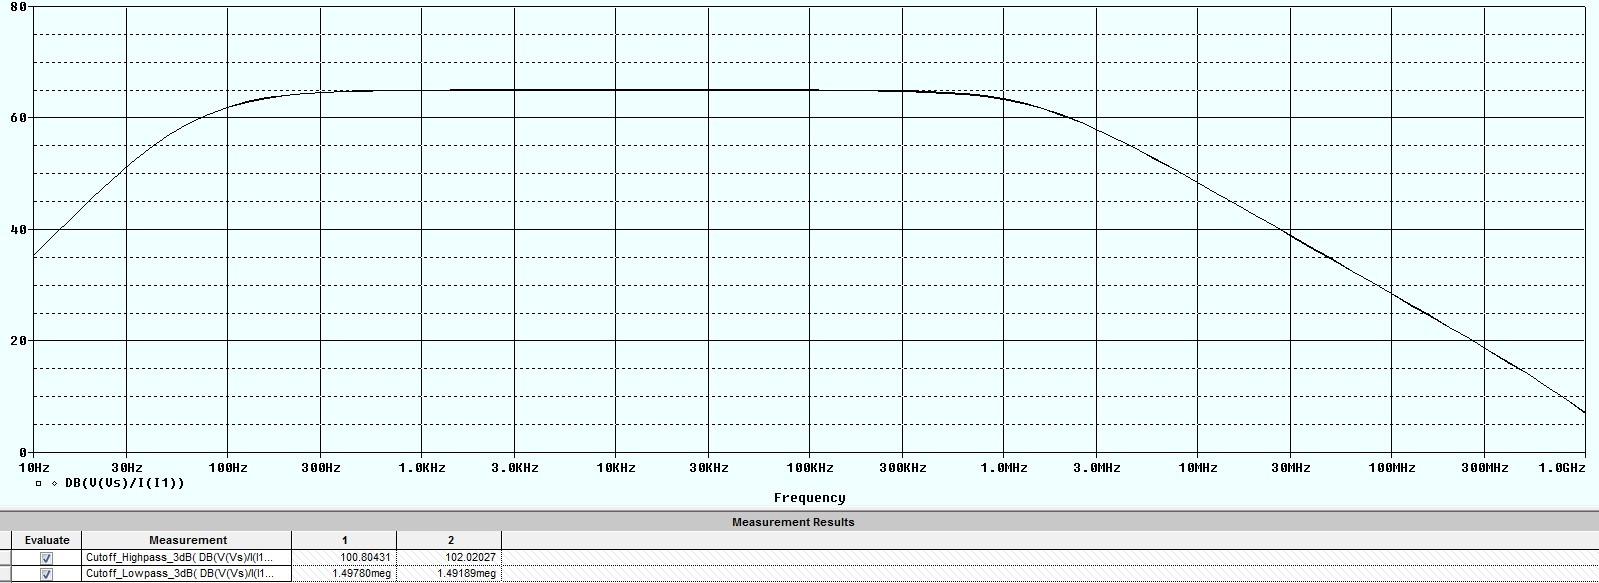
\includegraphics[width=\linewidth]{bode_res_serie_condo.jpg}

%On remplace donc ce condensateur par un circuit RLC série, qui résonne à 2MHz, d’après la datasheet. Ça nous donne une inductance de $\left(\cfrac{1}{2\pi 2 \cdot 10^6}\right)^2\cdot\cfrac{1}{330\cdot 10^{-6}} = 19 $pH.
%La datasheet nous donnait également une résistance de 50 mΩ à cette fréquence de résonnance, ce qui est donc la valeur de la résistance série du modèle équivalent.

De la même manière, pour l’autre condensateur, on choisit le BFC233860563, qui a une ESR 40mΩ, et dont l’ESL est de 9.23nH:

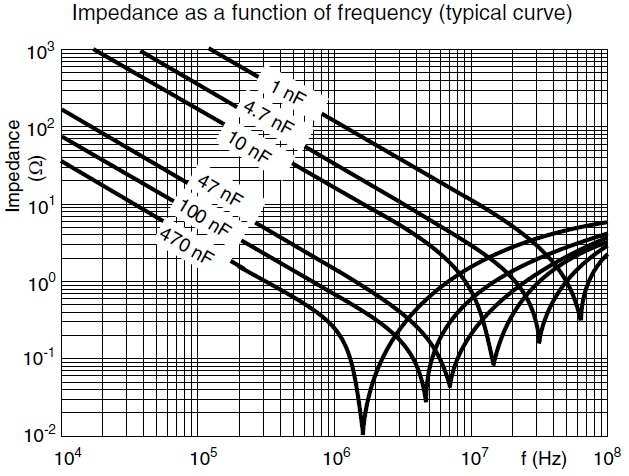
\includegraphics[width=\linewidth]{courbes_condo.jpg}

%Notre diagramme de Bode présente alors une résonnance assez prononcée:

On remarque alors que la fréquence de coupure basse a à nouveau augmenté:

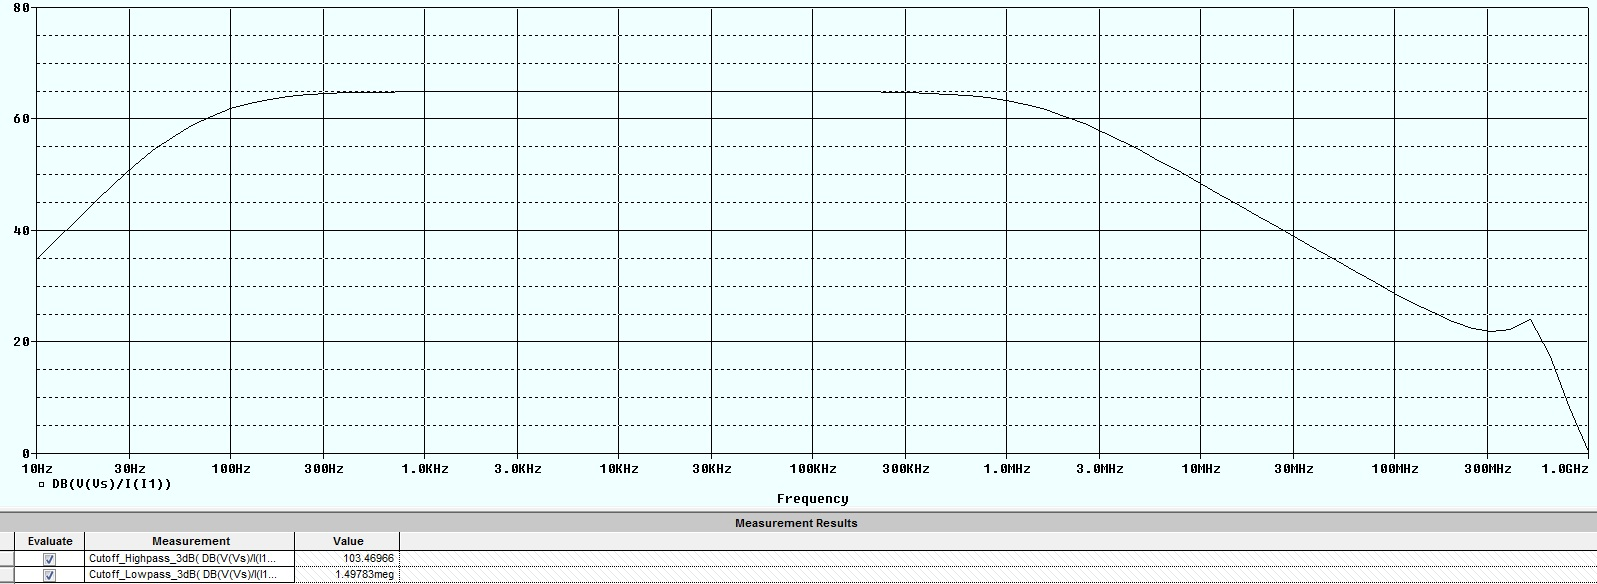
\includegraphics[width=\linewidth]{bode_LSR.jpg}

%De plus, la fréquence de coupure haute est abaissée d’une décade à cause de cette résonnance, ce qui nous montre que la seule utilisation de ces condensateurs ne nous permet plus de répondre au cahier des charges.

~

Cependant, il est fort probable que le choix d’autres condensateurs aurait entraîné des résultats différent, et c’est tout l’intérêt de cette étude.

\section{Modélisation d’une alimentation non-idéale}

L’alimentation n’est jamais idéale, il nous faut donc étudier l’impact de sa variation sur la sortie de notre système.

Pour cela, il suffit de tracer un diagramme de Bode:

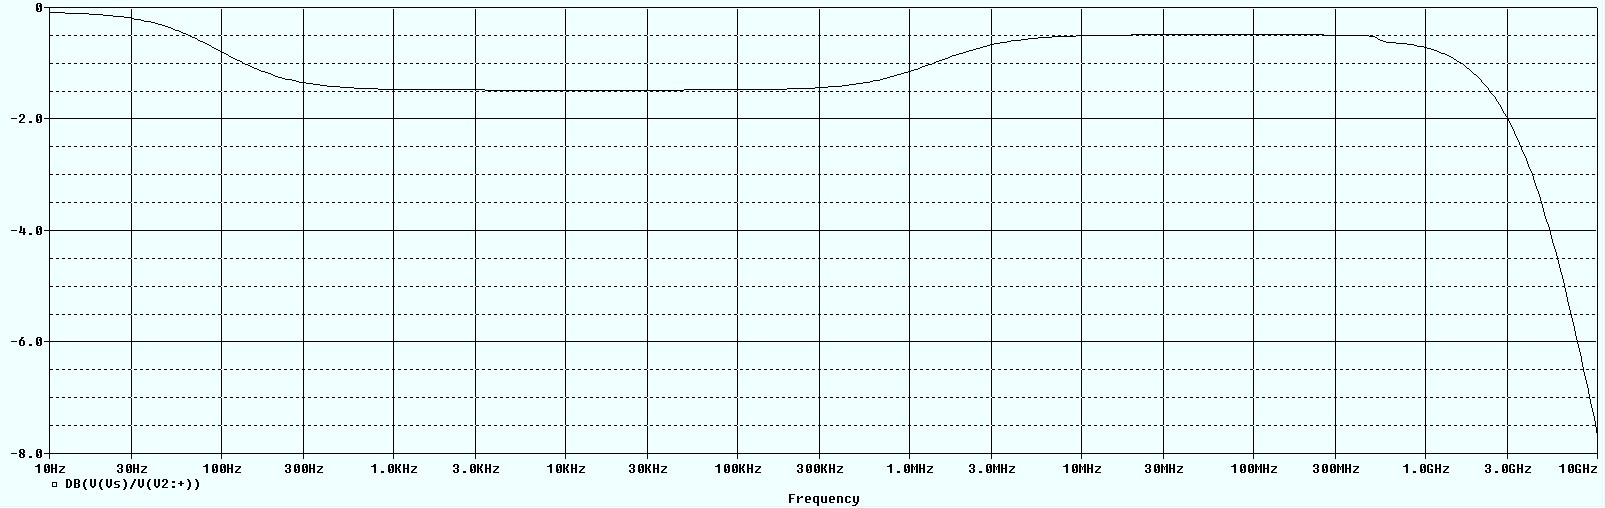
\includegraphics[width=\linewidth]{bode_alim.jpg}

Effectivement, l’impact d’une variation sur la tension d’alimentation est restituée de manière relativement peu atténuée sur la sortie. On retrouvera donc forcément un bruit sur notre montage, à moins d’ajouter des capacités de découplage.

\section{Modélisation des fils d’alimentation}

Si l’impact de l’alimentation est si important, il est intéressant de regarder l’impact des simples fils qui amènent l’alimentation au circuit.

On calcule que des fils de 10cm et d’1mm de diamètre ont une inductance de 105nH

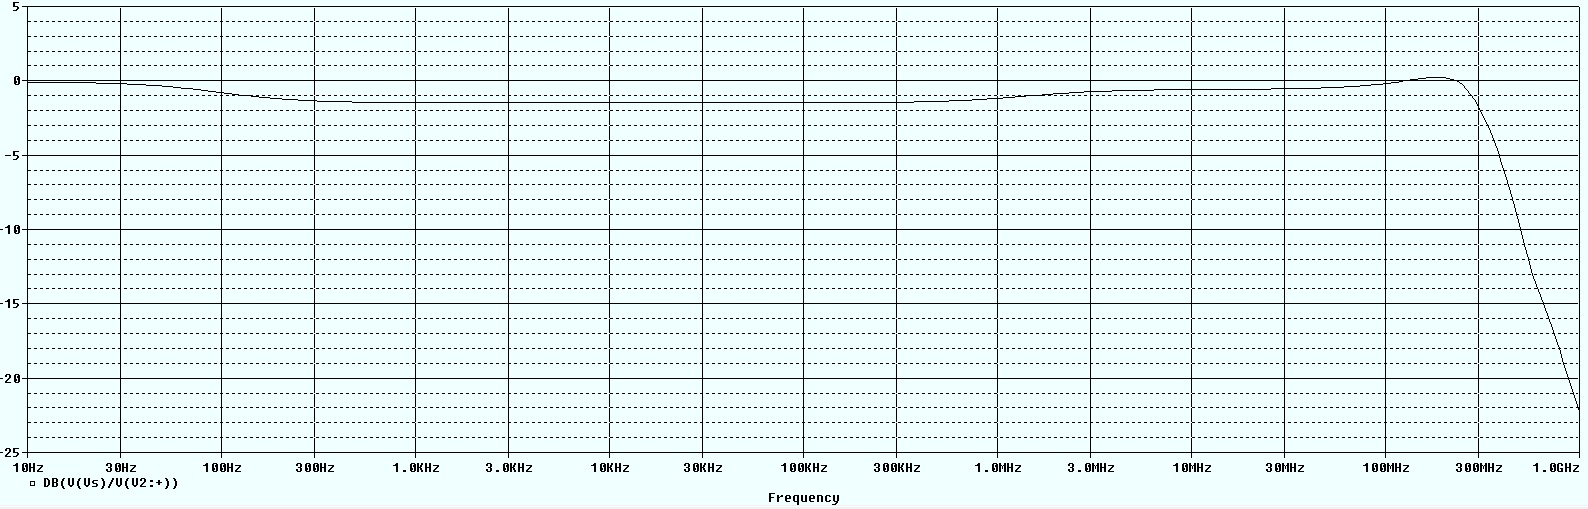
\includegraphics[width=\linewidth]{bode_alim_fil_reel.jpg}

L’impact de ces inductances parasites se fait essentiellement sentir au delà du GHz, donc hors de notre bande passante.

\section{Ajout de capacités de découplage}

Pour finir, après avoir vu que l’impact de l’alimentation était prépondérant, on essaye d’ajouter une capacité de découplage:

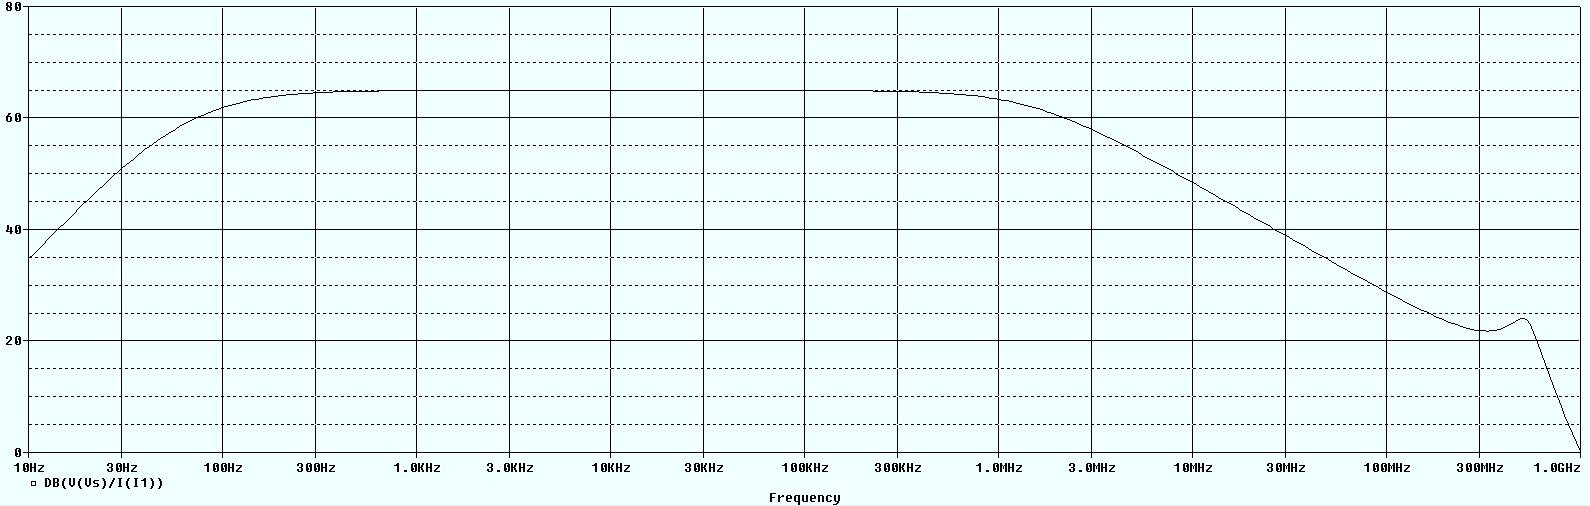
\includegraphics[width=\linewidth]{bode_alim_fil_reel_decouple.jpg}

\section*{Conclusion}

On a vu que dans certains cas, la modélisation des composants non idéaux nous montre qu’il est important de s’intéresser à l’impact du bruit sur notre circuit, même s’il n’a qu’un étage et est plutôt basique.

On distingue alors trois cas :
\begin{itemize}
    \item le passage en composants non idéaux n’a aucun impact;
    \item le passage en composants non idéaux a un impact hors de la bande passante;
    \item le passage en composants non idéaux a un impact dans de la bande passante;
\end{itemize}

Dans ce dernier cas, on peut alors facilement vérifier l’intérêt de l’ajout d’autres composants dont le but est de contrer les effets néfastes du bruit.

\end{document}
